%!TEX root = mainfile.tex

\newpage
\section{Calculating the Timescale of Reionization} % (fold)
\label{sec:calculating_the_timescale_of_reionization}
(Owen with contributions from Lewis)

	In the ``dark ages'' of the universe, when the universe had cooled, and matter had recombined to form neutral hydrogen, the temperature was not high enough to excite either hydrogen or helium out of the ground state, and consequently neither cooled effectively via atomic line emission. Thus no photon had sufficient energy to ionize neutral hydrogen.

	As stars began forming, the internal temperature of the gas was high enough for atomic line emission to occur, and ionizing photons were produced. At a particular redshift the star formation rate density was great enough to overcome the recombination rate. The star formation rate density at this point corresponds to the \emph{critical star formation rate density}. The star formation rate decreases with redshift, and conversely, the critical star formation rate increases, due to it proportionality with the clumping factor, Section~\ref{sec:clumping_factor}.

	\subsection{Critical Star Formation Rate Density} % (fold)
	\label{sub:critical_star_formation_rate_density}
		The critical star formation rate density was found by an analytical model, given by the following formula\cite{Pawlik:2009ij}.
		\begin{align}
			\rho^*_\text{SFR} = 0.027 \times f^{-1}_\text{esc} \left (\frac{C}{30} \right ) \left (\frac{1+z}{7} \right )^3 \left (\frac{\Omega_b h^2}{0.0465} \right )^2 (M_\odot \text{yr}^{-1} \text{Mpc}^{-3})
		\end{align}
		where $z$ is the redshift, $\Omega_b$ is the baryonic mass density and $C$ is the clumping factor. The graph of $\rho^*_\text{SFR}$ was plotted see Figure~\ref{fig:GRAPH_SFR_Density}.
		\begin{figure}[htbp]
			\centering
				\begingroup\endlinechar=-1
					\resizebox{0.8\textwidth}{!}{%
						% GNUPLOT: LaTeX picture with Postscript
\begingroup
  \makeatletter
  \providecommand\color[2][]{%
    \GenericError{(gnuplot) \space\space\space\@spaces}{%
      Package color not loaded in conjunction with
      terminal option `colourtext'%
    }{See the gnuplot documentation for explanation.%
    }{Either use 'blacktext' in gnuplot or load the package
      color.sty in LaTeX.}%
    \renewcommand\color[2][]{}%
  }%
  \providecommand\includegraphics[2][]{%
    \GenericError{(gnuplot) \space\space\space\@spaces}{%
      Package graphicx or graphics not loaded%
    }{See the gnuplot documentation for explanation.%
    }{The gnuplot epslatex terminal needs graphicx.sty or graphics.sty.}%
    \renewcommand\includegraphics[2][]{}%
  }%
  \providecommand\rotatebox[2]{#2}%
  \@ifundefined{ifGPcolor}{%
    \newif\ifGPcolor
    \GPcolortrue
  }{}%
  \@ifundefined{ifGPblacktext}{%
    \newif\ifGPblacktext
    \GPblacktexttrue
  }{}%
  % define a \g@addto@macro without @ in the name:
  \let\gplgaddtomacro\g@addto@macro
  % define empty templates for all commands taking text:
  \gdef\gplbacktext{}%
  \gdef\gplfronttext{}%
  \makeatother
  \ifGPblacktext
    % no textcolor at all
    \def\colorrgb#1{}%
    \def\colorgray#1{}%
  \else
    % gray or color?
    \ifGPcolor
      \def\colorrgb#1{\color[rgb]{#1}}%
      \def\colorgray#1{\color[gray]{#1}}%
      \expandafter\def\csname LTw\endcsname{\color{white}}%
      \expandafter\def\csname LTb\endcsname{\color{black}}%
      \expandafter\def\csname LTa\endcsname{\color{black}}%
      \expandafter\def\csname LT0\endcsname{\color[rgb]{1,0,0}}%
      \expandafter\def\csname LT1\endcsname{\color[rgb]{0,1,0}}%
      \expandafter\def\csname LT2\endcsname{\color[rgb]{0,0,1}}%
      \expandafter\def\csname LT3\endcsname{\color[rgb]{1,0,1}}%
      \expandafter\def\csname LT4\endcsname{\color[rgb]{0,1,1}}%
      \expandafter\def\csname LT5\endcsname{\color[rgb]{1,1,0}}%
      \expandafter\def\csname LT6\endcsname{\color[rgb]{0,0,0}}%
      \expandafter\def\csname LT7\endcsname{\color[rgb]{1,0.3,0}}%
      \expandafter\def\csname LT8\endcsname{\color[rgb]{0.5,0.5,0.5}}%
    \else
      % gray
      \def\colorrgb#1{\color{black}}%
      \def\colorgray#1{\color[gray]{#1}}%
      \expandafter\def\csname LTw\endcsname{\color{white}}%
      \expandafter\def\csname LTb\endcsname{\color{black}}%
      \expandafter\def\csname LTa\endcsname{\color{black}}%
      \expandafter\def\csname LT0\endcsname{\color{black}}%
      \expandafter\def\csname LT1\endcsname{\color{black}}%
      \expandafter\def\csname LT2\endcsname{\color{black}}%
      \expandafter\def\csname LT3\endcsname{\color{black}}%
      \expandafter\def\csname LT4\endcsname{\color{black}}%
      \expandafter\def\csname LT5\endcsname{\color{black}}%
      \expandafter\def\csname LT6\endcsname{\color{black}}%
      \expandafter\def\csname LT7\endcsname{\color{black}}%
      \expandafter\def\csname LT8\endcsname{\color{black}}%
    \fi
  \fi
  \setlength{\unitlength}{0.0500bp}%
  \begin{picture}(7200.00,4320.00)%
    \gplgaddtomacro\gplbacktext{%
      \put(849,595){\makebox(0,0)[r]{\strut{} 0}}%
      \put(849,1098){\makebox(0,0)[r]{\strut{} 0.02}}%
      \put(849,1601){\makebox(0,0)[r]{\strut{} 0.04}}%
      \put(849,2104){\makebox(0,0)[r]{\strut{} 0.06}}%
      \put(849,2606){\makebox(0,0)[r]{\strut{} 0.08}}%
      \put(849,3109){\makebox(0,0)[r]{\strut{} 0.1}}%
      \put(849,3612){\makebox(0,0)[r]{\strut{} 0.12}}%
      \put(849,4115){\makebox(0,0)[r]{\strut{} 0.14}}%
      \put(951,409){\makebox(0,0){\strut{} 0}}%
      \put(1941,409){\makebox(0,0){\strut{} 5}}%
      \put(2932,409){\makebox(0,0){\strut{} 10}}%
      \put(3922,409){\makebox(0,0){\strut{} 15}}%
      \put(4912,409){\makebox(0,0){\strut{} 20}}%
      \put(5903,409){\makebox(0,0){\strut{} 25}}%
      \put(6893,409){\makebox(0,0){\strut{} 30}}%
      \csname LTb\endcsname%
      \put(144,2355){\rotatebox{-270}{\makebox(0,0){\strut{}Star Formation Rate Density)}}}%
      \csname LTb\endcsname%
      \put(3922,130){\makebox(0,0){\strut{}Redshift ($z$)}}%
      \put(3922,4022){\makebox(0,0){\strut{}}}%
    }%
    \gplgaddtomacro\gplfronttext{%
    }%
    \gplbacktext
    \put(0,0){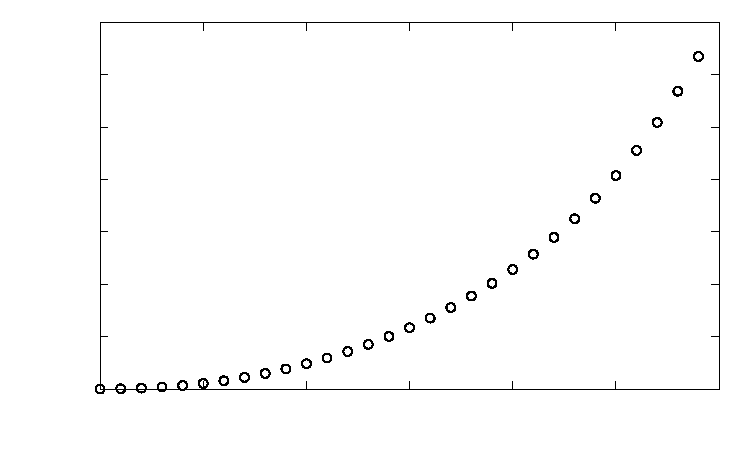
\includegraphics{GRAPH_SFR_Density}}%
    \gplfronttext
  \end{picture}%
\endgroup

					}\endgroup
			\caption{Graph of star formation rate density with redshift.\label{fig:GRAPH_SFR_Density}}
		\end{figure}
	% subsection critical_star_formation_rate_density (end)

	\subsection{Star Formation Rate Density} % (fold)
	\label{sub:star_formation_rate_density}
		The star formation rate density was approximated from the luminosity density, as per Equation~(\ref{eq:sfr_estimate})\cite{interactions_and_Induced_Star_Formation}
		\begin{align}
			\rho_\text{SFR}(M_\odot yr^{-1} Mpc^{-3})=1\times 10^{-28} \rho_L \label{eq:sfr_estimate}
		\end{align}
		where $\rho_L$ is spectral luminosity density in the region of $2150\pm 650 \AA$ in units of \si{\erg\per\second\per\hertz\per\cubic\mega\parsec}. Within this region it was assumed that the spectral luminosity density is constant. It was calculated from the integral of the Schechter function, multiplied by the luminosity, in terms of spectral luminosities. Since the characteristic magnitude parameters of the Schechter function were obtained in terms of AB Magnitudes, a conversion between AB Magnitudes and Spectral Luminosities was used.
		\begin{align}
			F_v = 10^{0.4(5-AB-48.6)}
		\end{align}
		Where $F_v$ is the Spectral Flux Density in units of \si{\erg\per\second\per\hertz\per\square\centi\metre} and AB is a monochromatic AB Magnitude see Appendix~\ref{sec:magnitude_to_spectral_luminosity}. This was used in conjunction with
		\begin{align}
			L_v=4\pi D_L^2 F_v
		\end{align}
		Where $L_v$ is a Spectral Luminosity in units of \si{\erg\per\second}, and $D_L$ if the luminosity distance of 10\,parsecs.	The lower luminosity limit on the Schechter function in Figure~\ref{fig:GRAPH_SFR_Density} corresponds to the spectral luminosity of galaxies with the smallest mass possible, discussed in Section~\ref{ssub:minimum_galaxy_mass}.

		\subsubsection{Minimum Galaxy Mass} % (fold)
		\label{ssub:minimum_galaxy_mass}
			In order to find the minimum mass, the redshift at which the Jeans mass (equation~\ref{eq:jeanssmass}) and the characteristic mass of a dark matter halo, (equation~(\ref{eq:characteristic_dark_halo}), were equal, was considered\cite{Barkana2001125}
			\begin{align}
				M^*=10^{13}h^{-1}(1+z)^{-4} M_\odot \label{eq:characteristic_dark_halo}
			\end{align}
			The Jeans Mass defines the critical mass of a cloud at which it will collapse to form a galaxy, thereby limiting the minimum mass of a star forming galaxy.\cite{Barkana2001125}.
			\begin{align}
				M_J \approx 5.73\times10^3 \left (\frac{1+z}{10} \right )^{3/2} M_{\odot} \label{eq:jeanssmass}
			\end{align}
			At the redshift at which these equations are equal, the mass of the galaxy was assumed to be separate and distinct from the rest of the mass of the universe. This assumption ensured that no additional matter could contribute to the mass of the gas after this point. The redshift at which this occurs was calculated to be z=106. This corresponds to a minimum mass of a galaxy of $M=1.1\times10^5M_\odot$.

			Adopting a Mass-Luminosity ratio of 1:1 for simplicity, the minimum mass was found to correspond to an upper limit on the luminosity of the galaxy of $1.1\times 10^5 L_\odot$. However this was a bolometric luminosity, representing power over all frequencies, as opposed to a spectral luminosity, the power at  a specific frequency. Thus, a conversion between bolometric luminosity and spectral luminosity was formulated.
		% subsubsection minimum_galaxy_mass (end)
	% subsection star_formation_rate_density (end)

		\subsection{Bolometric Luminosity to Spectral Luminosity} % (fold)
		\label{sub:bolometric_luminosity_to_spectral_luminosity}
			In order to deduce a relation between bolometric luminosity and spectral luminosity, it was necessary to approximate the shape of the spectrum of a typical galaxy. A blackbody spectrum of temperature $1\times 10^5$K. was used to represent this spectrum, as this temperature corresponds to the temperature of a source emitting at \SI{2150}{\angstrom} using
			\begin{align}
				\frac{3}{2}kT=hv
			\end{align}
			where $k$ is the Boltzmann Constant, $T$ is the temperature (K), $h$ is the Planck's constant and $v$ is frequency (Hz). As spectral luminosity is luminosity per unit frequency, it can be written that
			\begin{align}
				\int^{\infty}_{-\infty}L_v \d{v} = \int^{\infty}_{0}L_v \d{v} = L_\text{Bol}
			\end{align}
			where $L_\text{Bol}$ is the bolometric luminosity, in units of \si{\erg\per\second}. The intensity of a blackbody is proportional to the spectral luminosity, at a constant solid angle and surface area, therefore it follows
			\begin{align}
				L_v &= kI(v,T) \\
				\int^{\infty}_{0}L_v \d{v} &= L_\text{bol} \\
				k\int^{\infty}_{0}I \d{v} &= L_\text{bol} \\
				L_v &= \frac{I(v,T)}{\int^{\infty}_{0}I \d{v}} \times L_{bol}
			\end{align}
			% where$k$ is a constant, and $I(v,T)$ is the intensity as a function of frequency and temperature. $L_\text{Bol}/k$ was computed to be \SI{75224.6}{\erg\per\second\per\omega\per\square\centi\metre}.
			\begin{align}
				I(v,T)=\frac{8\pi v^2}{c^3}\frac{hv}{e^\frac{hv}{kT}-1}
			\end{align}
			where, within $I(v,T)$, $v$ is the frequency in Hertz corresponding to $2150\pm 650$ \AA, and $T=1.1\times 10^5$K. The lower limit of spectral luminosity in the UV range, corresponding to 2150\AA, therefore, was calculated to be $L_v =9.755\times 10^{21}$\,\si{\erg\per\second\per\hertz}.
		% subsection bolometric_luminosity_to_spectral_luminosity (end)

		\subsection{Upper Redshift Limit of Reionization} % (fold)
		\label{sub:upper_redshift_limit_of_reionization}
			In order to compute the luminosity density, it was necessary to convert the Schechter function integral into a gamma function. See Appendix~\ref{sec:schechter_function_to_gamma_function}. This permitted the actual star formation rate density to be computed. Subsequently both star formation rate density and critical star formation rate density were plotted against redshift in Figure~\ref{fig:GRAPH_SFR_CriticalSFR}.
			\begin{figure}[htbp]
				\centering
					\begingroup\endlinechar=-1
						\resizebox{0.8\textwidth}{!}{%
							% GNUPLOT: LaTeX picture with Postscript
\begingroup
  \makeatletter
  \providecommand\color[2][]{%
    \GenericError{(gnuplot) \space\space\space\@spaces}{%
      Package color not loaded in conjunction with
      terminal option `colourtext'%
    }{See the gnuplot documentation for explanation.%
    }{Either use 'blacktext' in gnuplot or load the package
      color.sty in LaTeX.}%
    \renewcommand\color[2][]{}%
  }%
  \providecommand\includegraphics[2][]{%
    \GenericError{(gnuplot) \space\space\space\@spaces}{%
      Package graphicx or graphics not loaded%
    }{See the gnuplot documentation for explanation.%
    }{The gnuplot epslatex terminal needs graphicx.sty or graphics.sty.}%
    \renewcommand\includegraphics[2][]{}%
  }%
  \providecommand\rotatebox[2]{#2}%
  \@ifundefined{ifGPcolor}{%
    \newif\ifGPcolor
    \GPcolortrue
  }{}%
  \@ifundefined{ifGPblacktext}{%
    \newif\ifGPblacktext
    \GPblacktexttrue
  }{}%
  % define a \g@addto@macro without @ in the name:
  \let\gplgaddtomacro\g@addto@macro
  % define empty templates for all commands taking text:
  \gdef\gplbacktext{}%
  \gdef\gplfronttext{}%
  \makeatother
  \ifGPblacktext
    % no textcolor at all
    \def\colorrgb#1{}%
    \def\colorgray#1{}%
  \else
    % gray or color?
    \ifGPcolor
      \def\colorrgb#1{\color[rgb]{#1}}%
      \def\colorgray#1{\color[gray]{#1}}%
      \expandafter\def\csname LTw\endcsname{\color{white}}%
      \expandafter\def\csname LTb\endcsname{\color{black}}%
      \expandafter\def\csname LTa\endcsname{\color{black}}%
      \expandafter\def\csname LT0\endcsname{\color[rgb]{1,0,0}}%
      \expandafter\def\csname LT1\endcsname{\color[rgb]{0,1,0}}%
      \expandafter\def\csname LT2\endcsname{\color[rgb]{0,0,1}}%
      \expandafter\def\csname LT3\endcsname{\color[rgb]{1,0,1}}%
      \expandafter\def\csname LT4\endcsname{\color[rgb]{0,1,1}}%
      \expandafter\def\csname LT5\endcsname{\color[rgb]{1,1,0}}%
      \expandafter\def\csname LT6\endcsname{\color[rgb]{0,0,0}}%
      \expandafter\def\csname LT7\endcsname{\color[rgb]{1,0.3,0}}%
      \expandafter\def\csname LT8\endcsname{\color[rgb]{0.5,0.5,0.5}}%
    \else
      % gray
      \def\colorrgb#1{\color{black}}%
      \def\colorgray#1{\color[gray]{#1}}%
      \expandafter\def\csname LTw\endcsname{\color{white}}%
      \expandafter\def\csname LTb\endcsname{\color{black}}%
      \expandafter\def\csname LTa\endcsname{\color{black}}%
      \expandafter\def\csname LT0\endcsname{\color{black}}%
      \expandafter\def\csname LT1\endcsname{\color{black}}%
      \expandafter\def\csname LT2\endcsname{\color{black}}%
      \expandafter\def\csname LT3\endcsname{\color{black}}%
      \expandafter\def\csname LT4\endcsname{\color{black}}%
      \expandafter\def\csname LT5\endcsname{\color{black}}%
      \expandafter\def\csname LT6\endcsname{\color{black}}%
      \expandafter\def\csname LT7\endcsname{\color{black}}%
      \expandafter\def\csname LT8\endcsname{\color{black}}%
    \fi
  \fi
  \setlength{\unitlength}{0.0500bp}%
  \begin{picture}(7200.00,4320.00)%
    \gplgaddtomacro\gplbacktext{%
      \put(849,595){\makebox(0,0)[r]{\strut{} 0}}%
      \put(849,1098){\makebox(0,0)[r]{\strut{} 0.05}}%
      \put(849,1601){\makebox(0,0)[r]{\strut{} 0.1}}%
      \put(849,2104){\makebox(0,0)[r]{\strut{} 0.15}}%
      \put(849,2606){\makebox(0,0)[r]{\strut{} 0.2}}%
      \put(849,3109){\makebox(0,0)[r]{\strut{} 0.25}}%
      \put(849,3612){\makebox(0,0)[r]{\strut{} 0.3}}%
      \put(849,4115){\makebox(0,0)[r]{\strut{} 0.35}}%
      \put(951,409){\makebox(0,0){\strut{} 10}}%
      \put(1545,409){\makebox(0,0){\strut{} 11}}%
      \put(2139,409){\makebox(0,0){\strut{} 12}}%
      \put(2734,409){\makebox(0,0){\strut{} 13}}%
      \put(3328,409){\makebox(0,0){\strut{} 14}}%
      \put(3922,409){\makebox(0,0){\strut{} 15}}%
      \put(4516,409){\makebox(0,0){\strut{} 16}}%
      \put(5110,409){\makebox(0,0){\strut{} 17}}%
      \put(5705,409){\makebox(0,0){\strut{} 18}}%
      \put(6299,409){\makebox(0,0){\strut{} 19}}%
      \put(6893,409){\makebox(0,0){\strut{} 20}}%
      \csname LTb\endcsname%
      \put(144,2355){\rotatebox{-270}{\makebox(0,0){\strut{}Star Formation Raet Density ($\M_\odot$\si{\per\year\per\cubic\mega\parsec})}}}%
      \csname LTb\endcsname%
      \put(3922,130){\makebox(0,0){\strut{}Redshift ($z$)}}%
      \put(3922,4022){\makebox(0,0){\strut{}}}%
    }%
    \gplgaddtomacro\gplfronttext{%
      \csname LTb\endcsname%
      \put(5910,3821){\makebox(0,0)[r]{\strut{}Critical SFR Density}}%
      \csname LTb\endcsname%
      \put(5910,3635){\makebox(0,0)[r]{\strut{}SFR Density}}%
    }%
    \gplbacktext
    \put(0,0){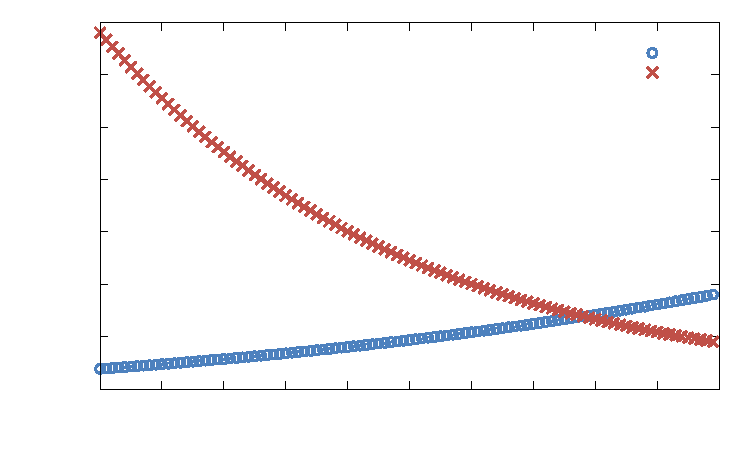
\includegraphics{GRAPH_SFR_CriticalSFR}}%
    \gplfronttext
  \end{picture}%
\endgroup

						}\endgroup
				\caption{Graph of star formation rate density and critical star formation rate.\label{fig:GRAPH_SFR_CriticalSFR}}
			\end{figure}

			As mentioned above the redshift at which the star formation rate density exceeds the critical star formation rate density will mark the beginning of reionization. This redshift corresponds to the point in Figure~\ref{fig:GRAPH_SFR_CriticalSFR}, where the two curves intersect. The resultant redshift was found to be $z = 17.82$. At high redshifts, low values of the $\phi^*$ parameter, and high values of the $M^*$ and $\alpha$ parameters result in a lower value of the Schechter function, and consequently the lower bound on redshift was calculated to be 15.42. Similarly, high values of the $\phi^*$ parameter, and low values of the $M^*$ and $\alpha$ parameters result in a higher value of the Schechter function integral, and consequently the upper bound on redshift was calculated to be 20.88.
		% subsection upper_redshift_limit_of_reionization (end)
% section calculating_the_timescale_of_reionization (end)
